

\subsection{The Physics GRE}


\subsection{Distribution of Topics}

\begin{figure}
    \centering
    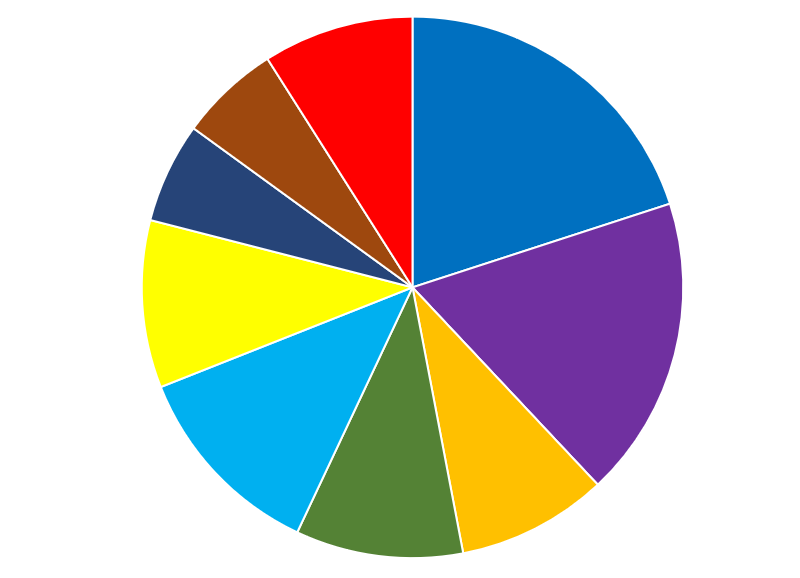
\includegraphics[width=8cm]{Introduction/topic-distribution.png}
    \caption{}
    \label{fig:topic-distribution}
\end{figure}

\begin{table}[h]
    \centering
        \begin{tabular}{ c c c } 
        %\multicolumn{3}{c}{{\large Topic Distribution}} \\
        %\hline
         20\% & Classical Mechanics & blue \\ 
         18\% & Electromagnetism & purple \\
         9\% & Optics \& Wave Phenomena & orange \\
         10\% & Thermodynamics \& Statistical Mechanics & green \\
         12\% & Quantum Mechanics & light blue \\
         10\% & Atomic Physics & yellow \\
         6\% & Special Relativity & dark blue \\
         6\% & Laboratory Methods & brown \\
         9\% & Specialized Topics & red \\
        \end{tabular}
    \caption{}
    \label{tab:distribution}
\end{table}


See Figure \ref{fig:topic-distribution} and Table \ref{tab:distribution} for topic distribution. See below for details on each topic.

\begin{itemize}
    \item {\bfseries Classical Mechanics}: kinematics, Newton's laws, work and energy, oscillatory motion, rotational motion about a fixed axis, dynamics of systems of particles, central forces and celestial mechanics, three-dimensional particle dynamics, Lagrangian and Hamiltonian formalism, noninertial reference frames, elementary topics in fluid dynamics.
    \item {\bfseries Electricity \& Magnetism}: electrostatics, currents and DC circuits, magnetic fields in free space, Lorentz force, induction, Maxwell's equations and their applications, electromagnetic waves, AC circuits, magnetic and electric fields in matter.
    
    \item {\bfseries Optics and Waves}: wave properties, superposition, interference, diffraction, geometrical optics, polarization, Doppler effect.
    
    \item {\bfseries Thermodynamics \& Statistical Mechanics}: the laws of thermodynamics, thermodynamic processes, equations of state, ideal gases, kinetic theory, ensembles, statistical concepts and calculation of thermodynamic quantities, thermal expansion and heat transfer.
    
    \item {\bfseries Quantum Mechanics}: fundamental concepts, solutions of the Schrödinger equation (including square wells, harmonic oscillators, and hydrogenic atoms), spin, angular momentum, wave function symmetry, elementary perturbation theory.
    
    \item {\bfseries Atomic Physics}: properties of electrons, Bohr model, energy quantization, atomic structure, atomic spectra, selection rules, black-body radiation, x-rays, atoms in electric and magnetic fields.
    
    \item {\bfseries Special Relativity}: introductory concepts, time dilation, length contraction, simultaneity, energy and momentum, four-vectors and Lorentz transformation, velocity addition.
    
    \item {\bfseries Laboratory Methods}: data and error analysis, electronics, instrumentation, radiation detection, counting statistics, interaction of charged particles with matter, lasers and optical interferometers, dimensional analysis, fundamental applications of probability and statistics
    
    \item {\bfseries Specialized Topics}: Nuclear and Particle physics (e.g., nuclear properties, radioactive decay, fission and fusion, reactions, fundamental properties of elementary particles), Condensed Matter (e.g., crystal structure, x-ray diffraction, thermal properties, electron theory of metals, semiconductors, superconductors), Miscellaneous (e.g., astrophysics, mathematical methods, computer applications)
\end{itemize}

\subsection{Resources}

{\bfseries Bold font items} were used. This list was adapted from {\itshape \bfseries Conquering the Physics GRE}, 3rd ed., by Kahn and Anderson.

\begin{enumerate}
    \item Classical Mechanics: 
    \begin{itemize}
        \item {\itshape \bfseries University Physics} any ed. by Young
        \item {\itshape Classical Dynamics of Particles and Systems} by S.T. Thornton \& J.B. Marion
        \item {\itshape \bfseries Classical Mechanics} by John Taylor
    \end{itemize}
    
    \item Electricity \& Magnetism: 
    \begin{itemize}
        \item {\itshape \bfseries University Physics} any ed. by Young for circuits
        \item {\itshape Electromagnetic Fields} by R.K. Wangsness for EM waves
        \item {\itshape Electricity \& Magnetism} by E. Purcell for basic physical concepts
        \item {\itshape \bfseries Introduction to Electrodynamics} by David Griffiths
    \end{itemize}
    
    \item Optics and Waves: 
    \begin{itemize}
        \item {\itshape \bfseries University Physics} any ed. by Young for most.
        \item {\itshape \bfseries Introduction to Electrodynamics} by David Griffiths 
    \end{itemize}
    
    \item Thermodynamics \& Statistical Mechanics: 
    \begin{itemize}
        \item {\itshape Thermal Physics} by C. Kittel
        \item {\itshape Elementary Statistical Physics} by C. Kittel
        \item {\itshape Fundamentals of Statistical and Thermal Physics} by F. Reif
        \item {\itshape Statistical Physics} by F. Mandl, decent pedagogy
        \item {\itshape Thermodynamics} by Fermi, good intro to basic concepts
    \end{itemize}
    
    \item Quantum Mechanics and Atomic Physics: 
    \begin{itemize}
        \item {\itshape \bfseries Introduction to Quantum Mechanics} by David Griffiths 
    \end{itemize}
    
    \item Special Relativity: 
    \begin{itemize}
        \item {\itshape \bfseries Introduction to Quantum Mechanics} by David Griffiths, Ch. 12
        \item {\itshape Introduction to Elementary Particles} by D. Griffiths, Ch. 3
    \end{itemize}
    
    \item Laboratory Methods: 
    \begin{itemize}
        \item {\itshape The Art of Electronics} by P. Horowitz and W. Hill, advanced circuitry
        \item {\itshape Radiation Detection and Measurement} by G.F. Knoll, general reference to radiation, Ch. 1, 2, 3, 4, and 10
        \item {\itshape Principles of Lasers} by O. Svelto, lasers
    \end{itemize}
    
    \item Specialized Topics: 
    \begin{itemize}
        \item {\itshape Introduction to Elementary Particles} by D. Griffiths, Ch. 1
        \item {\itshape Introduction to Solid State Particle Physics} by C. Kittel, condensed matter
        \item {\itshape Solid State Physics} by N. Ashcroft and N. Mermin, Ch. 1-9, condensed matter
    \end{itemize}
    
    \item All Around: 
    \begin{itemize}
        \item {\itshape Physics: A Student Companion} by L. Kirkby, distilled but wide-ranging
        \item {\itshape Introduction to Elementary Particles} by D. Griffiths, Ch. 3
    \end{itemize}
    
    \item Websites:
    \begin{itemize}
        \item www.grephysics.net - compilation of problems with student solutions.
        \item www.physicsgre.org - forum for discussion.
        \item www.aps.org/careers/guidance/webinars/gre-strategies.cfm - webinar on physics GRE prep.
    \end{itemize}
\end{enumerate}